
\documentclass[letterpaper]{article}
\usepackage{natbib,alifeconf}
\usepackage[hyphens]{url}
\usepackage{hyperref,booktabs,amsmath,array}
\hypersetup{hidelinks}

\newcommand\blfootnote[1]{%
  \begingroup
  \renewcommand\thefootnote{}\footnote{#1}%
  \addtocounter{footnote}{-1}%
  \endgroup
}

\title{Unbundling Affect-Coupled Control in an Inspectable ALife Agent:\\Readout and Modulation Support Distinct Behavioral Signatures}

\author{
Aishik Sanyal$^{1}$ \\
\mbox{}\\
$^1$ xcellect, Canada \\
\texttt{aishik@xcellect.com}
}

\begin{document}
\maketitle

\begin{abstract}
Artificial life models often invite psychological language, but tunability makes it unclear which architectural commitments actually support those descriptions. This paper extends ReCoN-Ipsundrum, an inspectable recurrent agent with affect-coupled control, by separating affective readout from affect-driven modulation of recurrent gain and precision. The extension adds multi-model support to the pain-tail assay, an ablation batch in the experiment runner, and a small analysis pipeline that compiles paper-facing summaries. Across four assays, the resulting decomposition is consistent. In familiarity control, the full and readout-only variants maintain high scenic-entry rates under novelty reversal (0.911 and 0.960), whereas modulation-only is lower (0.878 to 0.858). In reward-free exploratory play, modulation-only yields the broadest coverage (155.3 unique viewpoints, occupancy entropy 5.84) but near-zero cycle structure (0.2), while readout-only yields the strongest cyclic local investigation (cycle score 9.9) at lower coverage. Lesion experiments show that post-lesion persistence is more strongly tied to modulation than readout (AUC drop 27.63 for full and modulation-only versus 19.65 for readout-only). Pain-tail results are more tentative but suggest a further split between internal residual activity and overt turning bias. The broader claim is philosophical as well as engineering: controlled tunability is not merely a nuisance to be controlled away, but the experimental resource that lets ALife models reveal which interpretations attach to which mechanisms.
\end{abstract}

Submission type: \textbf{Full Paper}\\
Data/Code available at:\\
\url{https://github.com/xcellect/recips}
\blfootnote{\textcopyright\ 2026 Aishik Sanyal. Published under a Creative Commons Attribution 4.0 International (CC BY 4.0) license.}

\section{Introduction}
Artificial life has long functioned as a form of philosophical experimentation. In Dennett's phrase, ALife can operate as ``philosophy by other means'': by building a system, one makes explanatory commitments concrete and testable \citep{Dennett1994ArtificialLifePhilosophy}. Braitenberg's vehicles remain the canonical minimal example: once a mechanism is specified, psychological descriptions can be elicited, compared, and sometimes deflated \citep{Braitenberg1984Vehicles}. Yet this same virtue creates a methodological tension. If the rules are explicit and adjustable, when should a behavioral pattern count as a finding rather than an artifact of arbitrary tuning? Pattee's classic distinction between simulation, realization, and theory already warned that ALife must take the epistemic status of its models seriously \citep{Pattee1989Simulations}.

This tension is especially sharp for work that borders on artificial consciousness or synthetic psychology. Recent indicator-based discussions stress that behavioral markers should be triangulated with mechanistic and causal evidence, because the same surface behavior can be supported by importantly different internal organizations \citep{ButlinEtAl2025Indicators}. My previous paper, \emph{ReCoN-Ipsundrum}, took a step in that direction by implementing a small, inspectable agent that combines a ReCoN message-passing backbone with an ipsundrum-style recurrent persistence loop and an optional Barrett-inspired affect layer \citep{BachHerger2015ReCoN,Humphrey2023Sentience,Barrett2017HowEmotions,Sanyal2026ReCoNIpsundrum}. In that setting, affect-coupled control stabilized scenic preference under novelty competition, yielded structured local scanning in exploratory play, and produced longer post-stimulus caution.

The present paper asks a narrower and more ALife-typical question: \emph{what part of that affect coupling actually matters?} Instead of introducing a new architecture, I exploit the model's tunability to split affect into two computational roles. The first is \emph{readout}: valence, arousal, and body-budget error directly enter policy scoring. The second is \emph{modulation}: affect changes recurrent gain and effective precision inside the ipsundrum loop. Because the architecture is inspectable and the code paths are explicit, these roles can be separated cleanly.

This turns the model into a small experimental philosophy instrument. Rather than debating in the abstract whether ``affect'' supports preference, play, or lingering caution, we can ask which couplings support which signatures. The answer matters not because these toy agents are conscious, but because it clarifies the relationship between form, function, parameters, and dynamics in a concrete ALife system. In this respect, the paper is aligned with a long ALife tradition of using simple systems to sharpen questions about organization, autonomy, and minimal cognition \citep{Beer2020Autopoiesis}.

\paragraph{Contributions.} This extension makes three contributions. First, it adds a mechanism-decomposition layer to the original ReCoN-Ipsundrum codebase by implementing readout-only and modulation-only affect variants across four assays. Second, it contributes lightweight engineering work needed to make that decomposition reproducible: multi-model pain-tail support, ablation hooks in the main experiment runner, and a summary script that converts raw outputs into paper-facing tables. Third, it advances a philosophical claim: in ALife, tunability can be treated as an epistemic resource rather than an embarrassment, because carefully chosen ablations reveal which interpretations are licensed by which mechanisms.

\section{Base Architecture and Extension Design}
ReCoN-Ipsundrum starts from a small ReCoN controller, a transparent message-passing network for sensorimotor script execution \citep{BachHerger2015ReCoN}. The original paper adds an ipsundrum loop that sustains sensory salience across time and, optionally, an affect layer inspired by constructionist ideas about valence and arousal as internal regulatory readouts \citep{Humphrey2023Sentience,Barrett2017HowEmotions,Sanyal2026ReCoNIpsundrum}. In the full model, affect does two jobs at once: it contributes evaluative signals to action scoring, and it modulates recurrent dynamics by adjusting loop gain and precision.

The extension implemented here separates those two jobs. In \textbf{readout-only}, affective variables are preserved as explicit policy inputs, but state-dependent modulation of recurrent gain and precision is disabled. In \textbf{modulation-only}, affect still alters gain and precision inside the recurrent loop, but the policy no longer scores predicted valence, arousal, or body-budget error directly. The \textbf{full} model keeps both routes active. The three-way comparison is therefore not ``affect versus no affect,'' but two different ways for affect to matter.

\begin{table}[t]
\centering
\small
\begin{tabular}{@{}p{0.24\linewidth}p{0.17\linewidth}p{0.17\linewidth}p{0.30\linewidth}@{}}
\toprule
Variant & \shortstack{Policy\\scores\\affect?} & \shortstack{Affect\\modulates\\loop?} & Working hypothesis \\
\midrule
Full & yes & yes & balanced evaluative stability and exploratory control \\
Readout-only & yes & no & stable preference without state-dependent loop retuning \\
Modulation-only & no & yes & altered exploration and persistence without evaluative scoring \\
\bottomrule
\end{tabular}
\caption{Mechanism split used in the extension. The change is minimal at the architectural level but conceptually strong: affective readout and affective modulation are no longer forced to travel together.}
\label{tab:variants}
\end{table}

The engineering work recorded in the repository's ALife extension notes is intentionally modest. First, \texttt{pain\_tail\_assay.py} was extended with a \texttt{--models} interface so that the ablation triplet can be run without a custom wrapper. Second, \texttt{run\_experiments.sh} was updated so the ablation batch now includes familiarity control, exploratory play, lesion, and pain-tail. Third, \texttt{analysis/alife\_mechanism\_decomposition.py} compiles the raw assay outputs into small summary tables and markdown notes. This is important to the philosophical point of the paper: the decomposition is not just a verbal reinterpretation of existing figures, but a reproducible branch in the experimental pipeline.

\section{Assays and Provenance}
I use four assays, all inherited from the original paper. \textbf{Familiarity control} probes scenic-over-dull choice after structured exposure and is the cleanest test of whether evaluative preference can survive novelty reversal. \textbf{Exploratory play} is reward-free and reports coverage, revisit structure, scanning, and loopiness. \textbf{Lesion} performs within-assay sham versus recurrent ablation to measure the persistence cost of removing feedback and integration. \textbf{Pain-tail} forces a brief hazard contact, removes the hazard, and then measures lingering internal and behavioral consequences.

The dedicated ALife extension batch uses the commands recorded in \texttt{ENGINEERING\_NOTES.md}: 10 seeds for familiarity, exploratory play, lesion, and pain-tail; five post-familiarization repeats; 200 exploratory-play steps; a 150-step lesion post-window; and a 200-step pain-tail post window. To keep the extension lightweight, I treat these 10-seed runs as the primary dataset for the new decomposition. For familiarity and exploratory play, I also checked the higher-N paper-profile ablations already stored in \texttt{results/ablations}. Those 20-seed cross-checks preserve the same ordering and therefore strengthen confidence that the extension is not merely a small-sample accident.

\begin{figure*}[t]
    \centering
    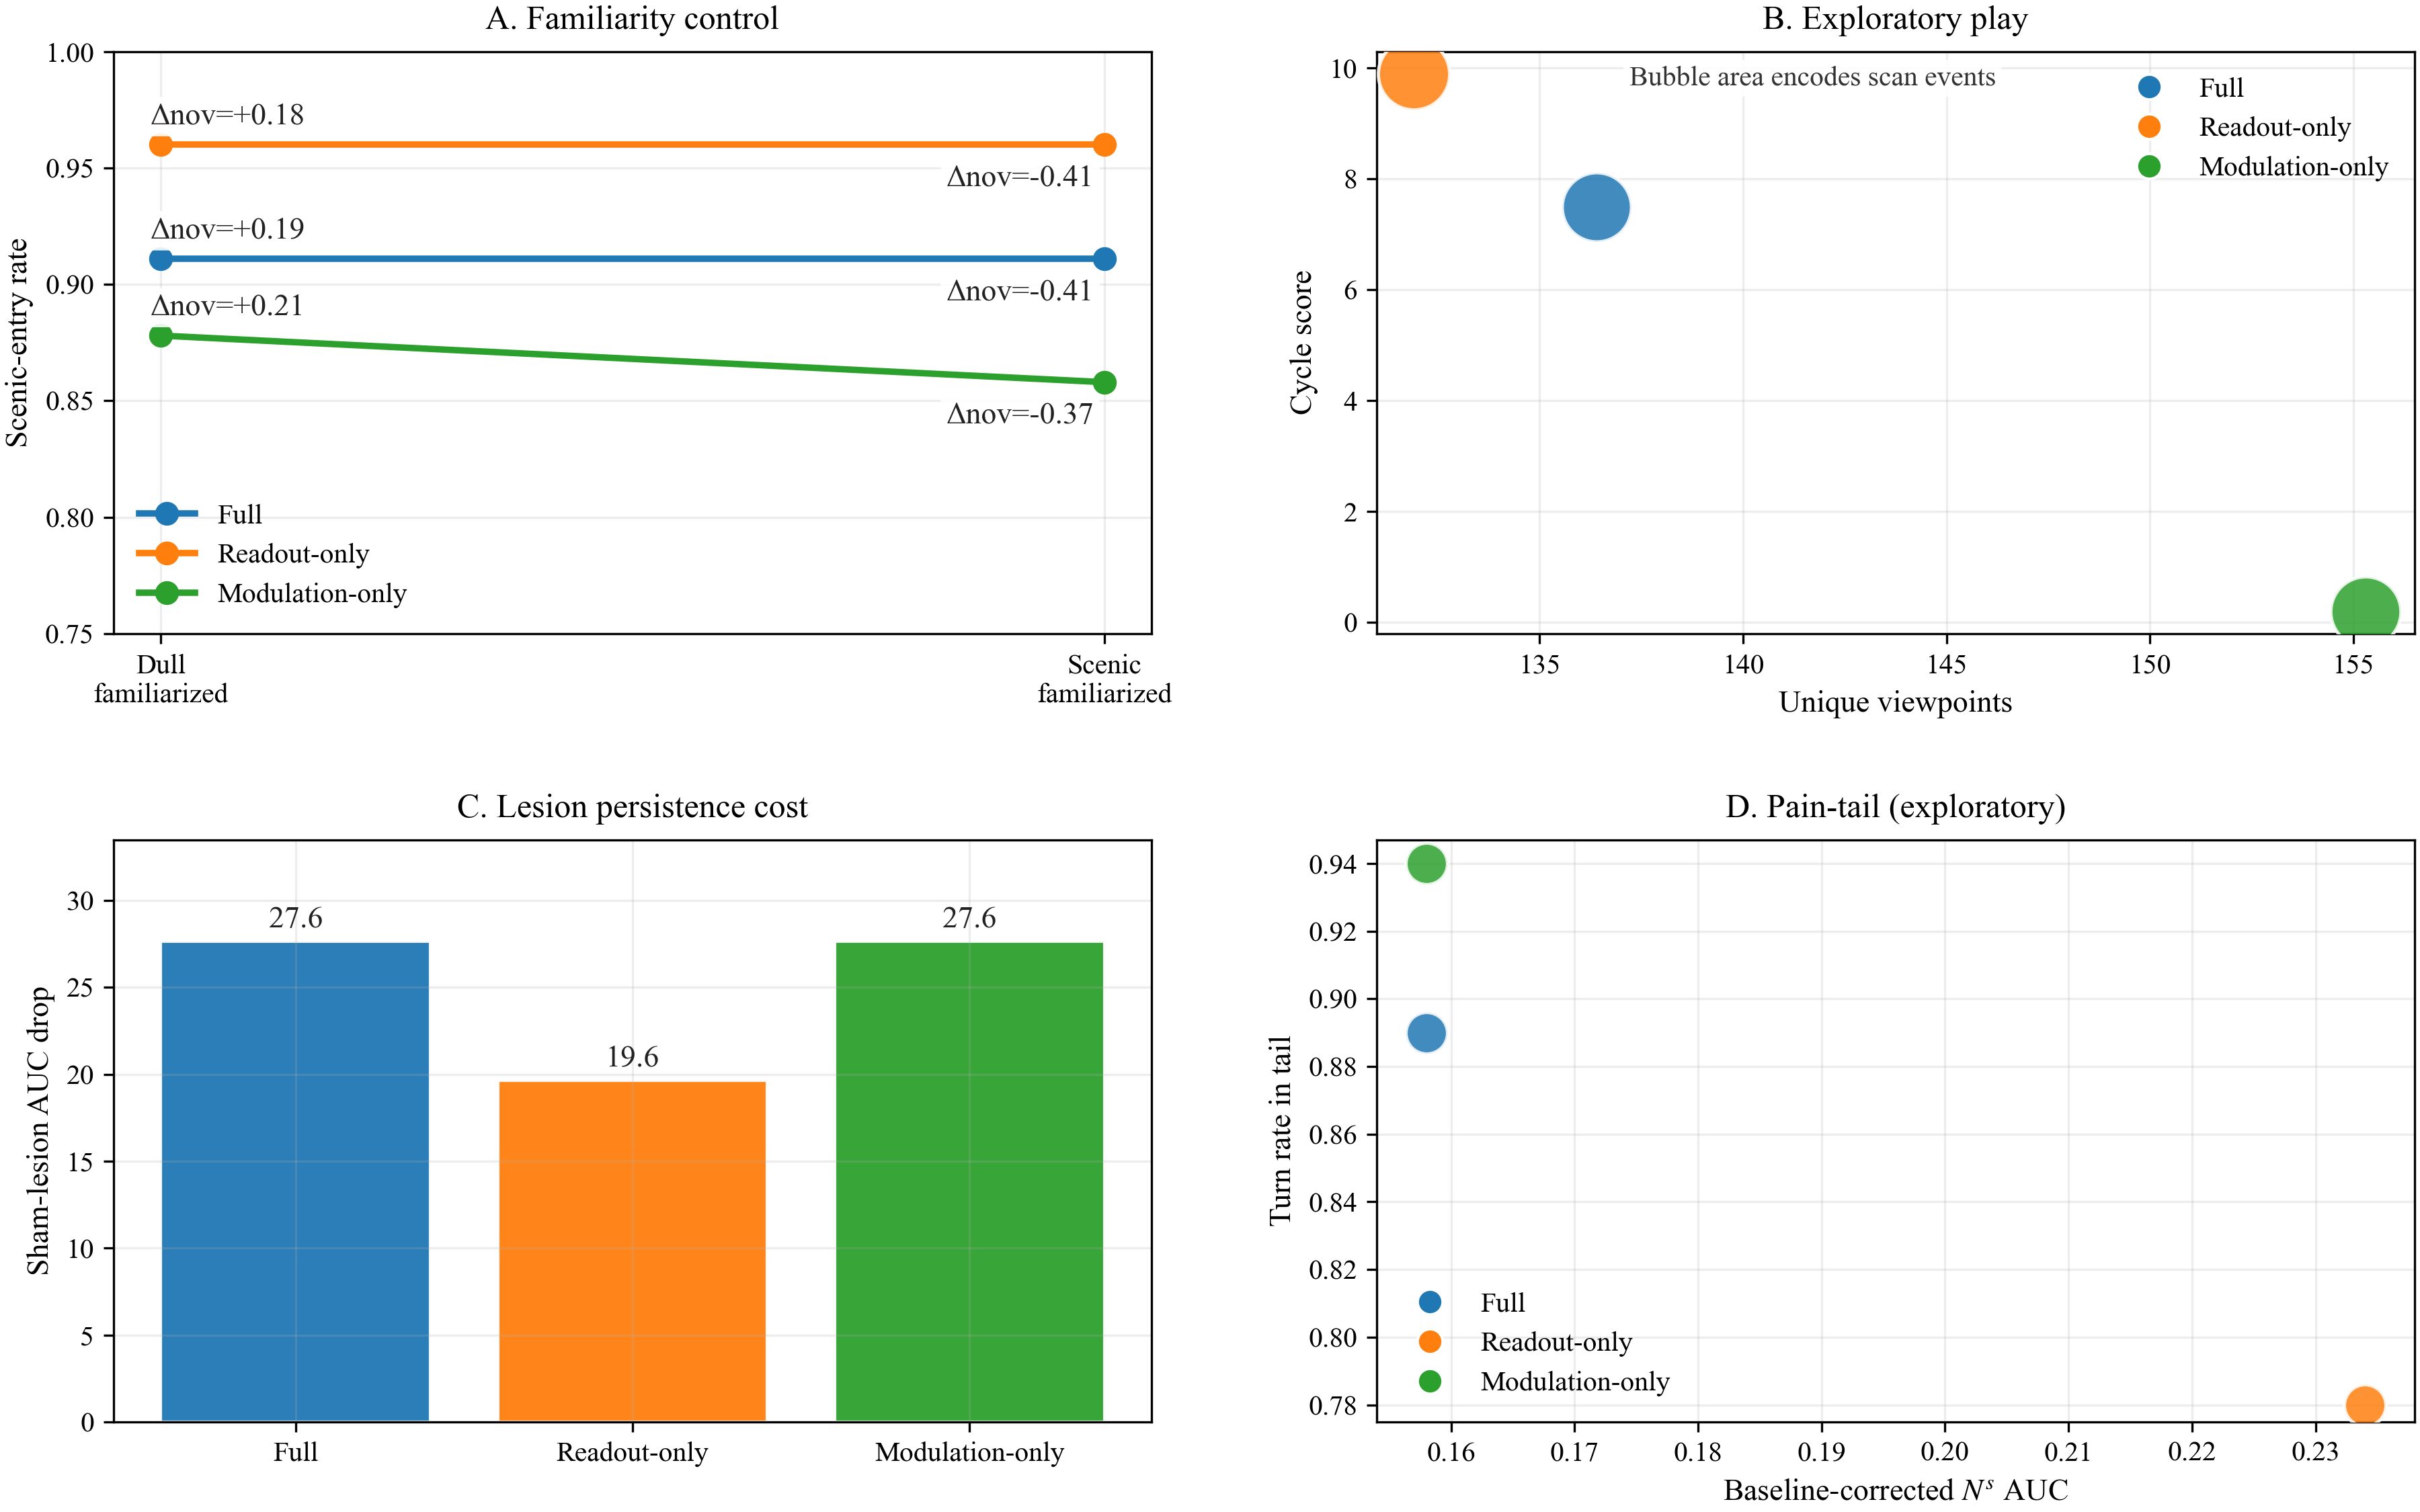
\includegraphics[width=0.96\textwidth]{fig_mechanism_decomposition.png}
    \caption{Mechanism decomposition across four assays. \textbf{A}: in familiarity control, full and readout-only remain stable even when familiarity reverses novelty, whereas modulation-only is weaker. \textbf{B}: in exploratory play, modulation-only maximizes coverage but loses cyclic local structure; readout-only preserves the strongest cycle score. \textbf{C}: sham-lesion AUC drop shows that recurrent persistence depends more strongly on modulation than on readout. \textbf{D}: pain-tail is exploratory but suggests another split: readout-only has the highest residual internal activity, while full and modulation-only show the strongest turning bias.}
    \label{fig:decomp}
\end{figure*}

\section{Results}
\subsection{Readout stabilizes route choice under novelty reversal}
The corridor assay provides the clearest evaluative result. In the dedicated extension batch, the full model sustains a scenic-entry rate of 0.911 whether the agent was previously familiarized with the dull or scenic side, even though the corresponding mean novelty difference flips from +0.186 to --0.405. Readout-only is even more stable: 0.960 in both conditions, with a comparable novelty reversal (+0.184 to --0.407). Modulation-only is lower and modestly more novelty-sensitive, dropping from 0.878 after dull familiarization to 0.858 after scenic familiarization.

This is the strongest evidence that evaluative \emph{readout} rather than recurrent \emph{modulation} is doing the main work in route-choice stability. Readout-only also yields the highest predicted scenic valence (0.819 versus 0.748 for full and 0.744 for modulation-only) and the lowest scenic arousal (0.084 versus 0.103 and 0.103), consistent with a policy that directly privileges positively evaluated trajectories instead of merely altering internal gain.

The higher-N paper-profile ablations in \texttt{results/ablations} preserve the same picture. There, weighted scenic-entry rates remain essentially unchanged between dull and scenic familiarization for full (0.956 versus 0.955) and readout-only (0.947 versus 0.946), while modulation-only stays lower overall (0.869 versus 0.857). The detailed values change with seed count, but the mechanism-level ordering is the same.

\subsection{Modulation broadens exploratory coverage, while readout preserves loopiness}
The exploratory-play assay reveals a different split. Modulation-only yields the broadest roaming: 155.3 unique viewpoints, revisit rate 0.2235, occupancy entropy 5.836, and scan events 34.8. In other words, it covers more of the arena and re-enters previous states less often. But this comes at the cost of local structure: its cycle score is only 0.2. Readout-only shows nearly the opposite profile: lower coverage (131.9 unique viewpoints), higher revisit rate (0.3405), but the strongest cycle score (9.9) and highest mean valence (0.559). The full model sits between those extremes, combining substantial scan events (33.9) with nontrivial cyclic structure (7.5).

This is a clean ALife decomposition result. ``Exploration'' is not one thing. If one uses coverage alone, modulation-only looks best. If one cares about local, repeatedly interrogative investigation---staying with a region and working it from multiple viewpoints---readout-only and the full model are better fits. The effect persists in the 20-seed \texttt{results/ablations} cross-check, where modulation-only again shows the greatest coverage (153.45) and readout-only the strongest cycle score (10.15).

\subsection{Lesions tie persistence more strongly to modulation than to readout}
The lesion assay is especially informative because it moves beyond descriptive behavior and directly perturbs the recurrence mechanism. Here the decomposition is strikingly asymmetric. Full and modulation-only are effectively identical: both have a sham-versus-lesion AUC drop of 27.63, with immediate slopes collapsing from approximately flat to strongly negative after the lesion. Readout-only is still lesion-sensitive, but substantially less so, with an AUC drop of 19.65.

The natural interpretation is that recurrent persistence is carried primarily by the modulation path, not by evaluative scoring. Readout can shape action choice and stabilize preference, but if one wants the loop itself to resist perturbation and sustain post-stimulus activity, state-dependent modulation matters more. This result is important philosophically because it shows that two traits that might both be described informally as ``affective''---evaluative preference and persistence of internal activity---attach to different couplings.

\subsection{Pain-tail is exploratory, but suggests a further split}
Pain-tail is the noisiest assay in the extension and should be treated cautiously. Tail durations are long and variable for all three variants (120.6--128.2 steps with standard deviations around 88--96), and the baseline-corrected half-life measure remains near zero because the trace rapidly returns to threshold. Even so, the assay is suggestive. Readout-only has the highest baseline-corrected Ns AUC (0.234 versus 0.158 for both full and modulation-only), yet it shows the weakest turning bias in the tail (0.78 turn rate versus 0.89 and 0.94) and the highest forward rate (0.22 versus 0.11 and 0.06).

Taken together, these numbers suggest that internal residual activity and overt motor caution can come apart. Readout-only retains more post-stimulus internal signal, but full and modulation-only translate the hazard encounter into stronger turning-heavy action selection. If this pattern survives a larger run, it would indicate that pain-tail behavior depends more on affective control modulation than on raw internal residue alone.

\section{Discussion}
The main lesson of this extension is methodological. In ALife, tunability is often treated defensively: a good result is supposed to be robust \emph{despite} the fact that parameters were chosen, couplings enabled, and scores weighted. Robustness does matter. But the present study shows that carefully constrained tunability is also what makes the system informative. By splitting a single architectural phrase---``affect-coupled control''---into two explicit routes, we learn that different behavioral descriptions attach to different mechanisms.

The decomposition is consistent across the four assays. Route-choice stability under novelty competition depends most strongly on evaluative readout. Recurrent persistence under lesion depends more strongly on modulation. Reward-free exploratory coverage is amplified by modulation, while locally cyclic and arguably more ``investigative'' play is strongest when readout is preserved. Pain-tail, although still exploratory, hints that internal residue and motor caution may be dissociable in the same way. The full model is therefore best understood not as a monolithic affective agent, but as a composition of separable functions whose joint operation produces the richer phenotype.

This matters for experimental philosophy because it changes how one should read small computational models. The value of the model is not that it settles whether affect, agency, or proto-consciousness is ``really present.'' It is that it lets us ask a finer-grained question: under what mechanistic interpretation does a given behavioral signature become intelligible? That is a characteristically ALife move. Rather than merely simulate a phenomenon, we intervene on the generative assumptions and observe which philosophical descriptions survive.

The paper also sharpens how the original ReCoN-Ipsundrum results should be interpreted. The earlier dissociation table treated affect-coupled control as a single explanatory block. The new ablations show that this is too coarse. If one were mapping the architecture to candidate indicators or synthetic-psychology vocabularies, one should say: evaluative preference is most closely tied to readout, broad exploratory state-space coverage to modulation, and recurrent persistence to the modulation-sensitive loop itself. Those are more defensible claims than a global assertion that ``affect'' explains all three.

\paragraph{Limitations.} The extension is intentionally fast. The dedicated mechanism-decomposition batch uses only 10 seeds, and pain-tail in particular remains noisy. The environments are stylized, the agents do not learn online, and the recurrent lesion is still a relatively blunt manipulation. For that reason, I treat pain-tail as exploratory and rely on the higher-N \texttt{results/ablations} runs as cross-checks for familiarity and play. Future work should rerun the full four-assay decomposition at the paper profile, add confidence intervals directly to the extension summaries, and test whether the readout/modulation split survives under other loop parameterizations.

\section{Conclusion}
This paper used a small engineering extension to turn ReCoN-Ipsundrum into a mechanism-decomposition experiment. Splitting affect into readout and modulation shows that the original ``affect-coupled'' signatures do not travel together: stable scenic preference attaches most strongly to readout, broad exploratory coverage and lesion sensitivity attach to modulation, and the full agent combines both routes. For ALife, the more general lesson is that tunability should not always be treated as a threat to findings. When couplings are explicit and ablations are inspectable, tunability becomes the means by which a model can function as experimental philosophy.

\footnotesize
\begin{thebibliography}{}

\bibitem[Bach and Herger(2015)]{BachHerger2015ReCoN}
Bach, J. and Herger, P. (2015).
\newblock Request confirmation networks for neuro-symbolic script execution.
\newblock In \emph{Proceedings of the Workshop on Cognitive Computation: Integrating Neural and Symbolic Approaches (CoCo@NIPS 2015)}.

\bibitem[Barrett(2017)]{Barrett2017HowEmotions}
Barrett, L.~F. (2017).
\newblock \emph{How Emotions Are Made: The Secret Life of the Brain}.
\newblock Houghton Mifflin Harcourt.

\bibitem[Beer(2020)]{Beer2020Autopoiesis}
Beer, R.~D. (2020).
\newblock An investigation into the origin of autopoiesis.
\newblock \emph{Artificial Life}, 26(1):5--22.

\bibitem[Braitenberg(1984)]{Braitenberg1984Vehicles}
Braitenberg, V. (1984).
\newblock \emph{Vehicles: Experiments in Synthetic Psychology}.
\newblock MIT Press.

\bibitem[Butlin et~al.(2025)]{ButlinEtAl2025Indicators}
Butlin, P., Long, R., Bayne, T., Bengio, Y., Birch, J., Chalmers, D., Constant, A., Deane, G., Elmoznino, E., Fleming, S.~M., Ji, X., Kanai, R., Klein, C., Lindsay, G., Michel, M., Mudrik, L., Peters, M.~A.~K., Schwitzgebel, E., Simon, J., and VanRullen, R. (2025).
\newblock Identifying indicators of consciousness in {AI} systems.
\newblock \emph{Trends in Cognitive Sciences}. Online ahead of print.

\bibitem[Dennett(1994)]{Dennett1994ArtificialLifePhilosophy}
Dennett, D.~C. (1994).
\newblock Artificial life as philosophy.
\newblock \emph{Artificial Life}, 1(3):291--292.

\bibitem[Humphrey(2023)]{Humphrey2023Sentience}
Humphrey, N. (2023).
\newblock \emph{Sentience: The Invention of Consciousness}.
\newblock MIT Press.

\bibitem[Pattee(1989)]{Pattee1989Simulations}
Pattee, H.~H. (1989).
\newblock Simulations, realizations, and theories of life.
\newblock In Langton, C.~G., editor, \emph{Artificial Life}, pages 63--77. Addison-Wesley.

\bibitem[Sanyal(2026)]{Sanyal2026ReCoNIpsundrum}
Sanyal, A. (2026).
\newblock ReCoN-Ipsundrum: An inspectable recurrent persistence loop agent with affect-coupled control and mechanism-linked consciousness indicator assays.
\newblock \emph{arXiv preprint arXiv:2602.23232}.

\end{thebibliography}

\end{document}
